\documentclass[border=10pt]{standalone}

\usepackage{tikz}
\usepackage{tikzsymbols}
\usetikzlibrary{calc,patterns,shapes.geometric}

\def\centerarc[#1](#2)(#3:#4:#5){\draw[#1] ($(#2)+({#5*cos(#3)},{#5*sin(#3)})$) arc (#3:#4:#5);}

\begin{document}
	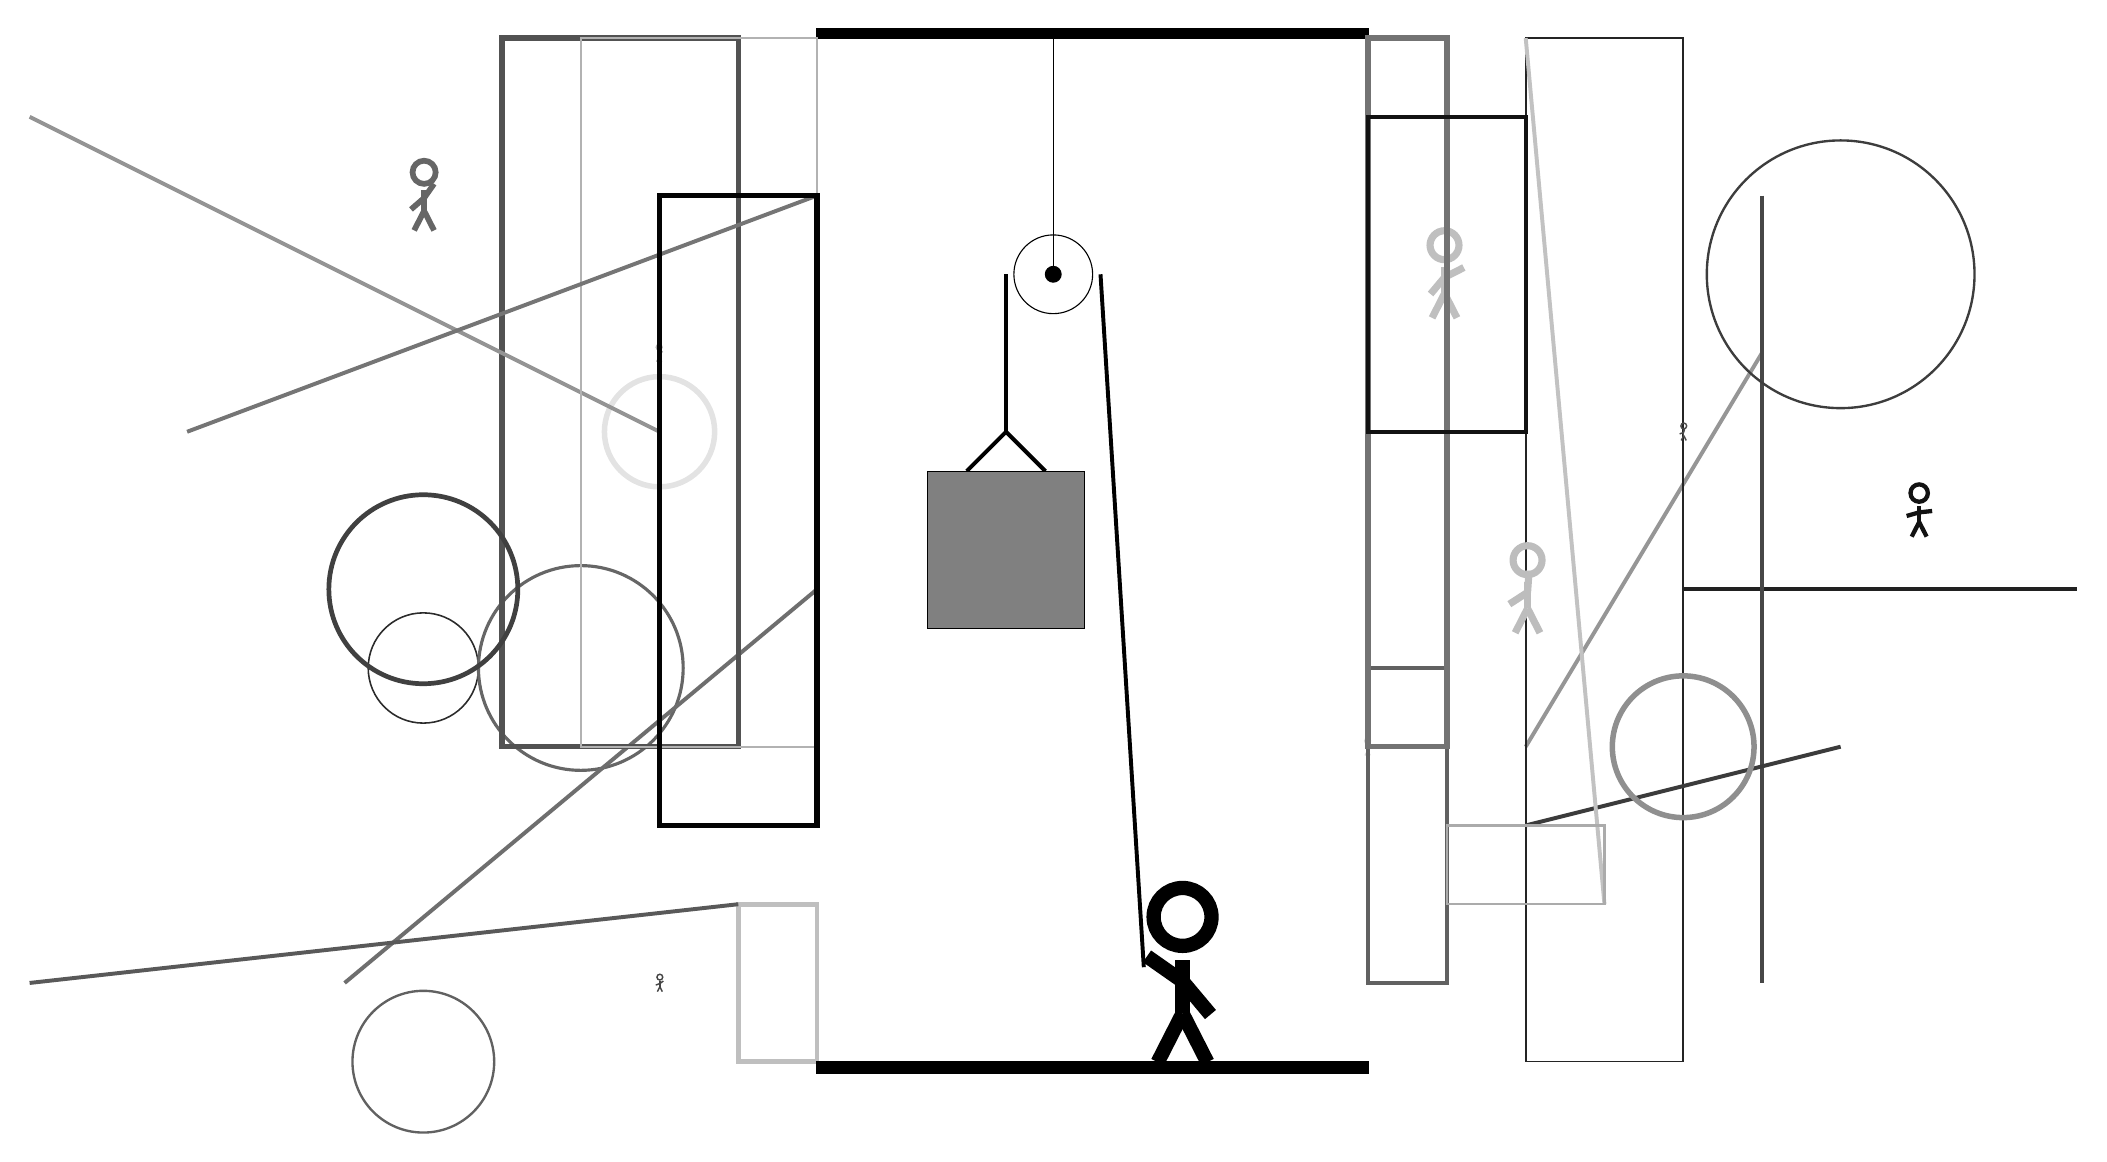
\begin{tikzpicture}
		%%%%% START %%%%%
		
		\draw[fill=black] (-2, 10) rectangle (5, 10.125);
		
		\draw[line width=0.6mm, color=black!25] (-2, -3) rectangle (-3, -1);
		
		\node[line width=0.2mm, color=black!25] at (6, 7) {\Strichmaxerl[5][50][27]};
		\node[line width=0.3mm, color=black!30] at (-4, 6) {\Strichmaxerl[1][89][31]};
		\draw [line width=0.2mm, color=black!83](-7, 2) circle (0.7);
		\draw [line width=0.7mm, color=black!11](-4, 5) circle (0.7);
		\draw [line width=0.4mm, color=black!60](-5, 2) circle (1.3);
		\draw[line width=0.5mm, color=black!41](7, 1) -- (10, 6);
		
		\draw[line width=0.5mm, color=black!87](9, 3) -- (14, 3);
		\node[line width=0.4mm, color=black!16] at (5, 1) {\Strichmaxerl[1][79][16]};
		
		\draw[line width=0.5mm, color=black!72](10, 8) -- (10, -2);
		\draw[line width=0.2mm, color=black!86] (7, 10) rectangle (9, -3);
		\draw[line width=0.5mm, color=black!62] (6, -2) rectangle (5, 2);
		\draw[line width=0.7mm, color=black!55] (5, 1) rectangle (6, 10);
		
		\node[line width=0.2mm, color=black!26] at (7, 3) {\Strichmaxerl[5][33][86]};
		\node[line width=0.4mm, color=black!71] at (9, 5) {\Strichmaxerl[1][20][78]};
		\draw[line width=0.6mm, color=black!26] (-2, 2) rectangle (-2, 4);
		
		\draw[line width=0.5mm, color=black!57](-2, 3) -- (-8, -2);
		\draw[line width=0.7mm, color=black!68] (-3, 1) rectangle (-6, 10);
		\draw[line width=0.5mm, color=black!77](7, 0) -- (11, 1);
		
		\draw [line width=0.7mm, color=black!44](9, 1) circle (0.9);
		\draw[line width=0.5mm, color=black!65](-3, -1) -- (-12, -2);
		
		\draw[line width=0.5mm, color=black!42](-4, 5) -- (-12, 9);
		
		\node[line width=0.6mm, color=black!73] at (-4, -2) {\Strichmaxerl[1][20][36]};
		\node[line width=0.4mm, color=black!60] at (-7, 8) {\Strichmaxerl[4][41][55]};
		\draw[line width=0.2mm, color=black!30] (-2, 1) rectangle (-5, 10);
		\draw[line width=0.5mm, color=black!24](7, 10) -- (8, -1);
		\draw[line width=0.5mm, color=black!54](-2, 8) -- (-10, 5);
		\node[line width=0.4mm, color=black!93] at (12, 4) {\Strichmaxerl[3][16][6]};
		\draw [line width=0.3mm, color=black!62](-7, -3) circle (0.9);
		\draw [line width=0.6mm, color=black!75](-7, 3) circle (1.2);
		\draw[line width=0.5mm, color=black!93] (5, 9) rectangle (7, 5);
		
		\draw [line width=0.3mm, color=black!76](11, 7) circle (1.7);
		\draw[line width=0.7mm, color=black!99] (-2, 8) rectangle (-4, 0);
		
		\draw[line width=0.3mm, color=black!33] (6, 0) rectangle (8, -1);
		
		\draw (1, 7) circle (0.5);
		\draw[fill=black] (1, 7) circle (0.1);
		\draw (1, 10) -- (1, 7);
		
		\draw[line width=0.5mm] (-0.1, 4.5) -- (0.4, 5.0) -- (0.9, 4.5);
		\draw[fill=black!50] (-0.6, 4.5) rectangle (1.4, 2.5);
		
		\draw[line width=0.5mm] (0.4, 7) -- (0.4, 5.0);
		\centerarc[line width=0.5mm](1, 7)(0:180:0.6);
		\draw[line width=0.5mm](1.6, 7) -- (2.15, -1.8);
		
		\node at (2.6, -1.9) {\Strichmaxerl[10][-35][-50]};
		
		\draw[fill=black] (-2, -3) rectangle (5, -3.15);
		
		%%%%% END %%%%%
	\end{tikzpicture}
\end{document}